\label{sec:arquitectura_sistema}

El sistema se organiza en cuatro bloques principales: \emph{nodo de sensado}, \emph{servicios backend}, \emph{procesamiento de audio} y \emph{aplicación cliente}. La comunicación se realiza de manera directa entre la aplicación móvil y los servicios, mediante consultas periódicas al servidor.

\begin{itemize}
    \item \textbf{Nodo de sensado (beehive-node):} Microcontrolador encargado de la captura de datos provenientes de la colmena, incluyendo sensores de temperatura, humedad, peso y audio.
    \item \textbf{Servicios backend:}
    \begin{itemize}
        \item \textit{beehive-guard:} gestiona la seguridad, autenticación y autorización de los usuarios; persiste en la base de datos \texttt{"guard-database"}.
        \item \textit{beehive-nest:} centraliza los metadatos de colmenas, sensores y registros; se conecta con la base de datos \texttt{"nest-database"}.
        \item \textit{beehive-mind:} ejecuta el modelo de aprendizaje automático para el análisis acústico; se apoya en la base de datos \texttt{"mind-database"}.
    \end{itemize}
    \item \textbf{Contenedor de audio (audio-container):} 
    se encarga de la persistencia de las grabaciones de audio mediante un 
    \emph{servicio de almacenamiento de objetos} compatible con la API S3. 
    De esta forma, los archivos no se gestionan en una base de datos relacional, 
    sino en depósitos lógicos denominados \emph{buckets}. 
    Para las pruebas se utilizó MinIO como implementación local de S3.
    \item \textbf{Aplicación móvil (beehive-app):} utilizada por el apicultor para visualizar información de las colmenas en tiempo real y recibir notificaciones. Interactúa directamente con los servicios backend mediante solicitudes periódicas.
\end{itemize}

Los flujos principales del sistema son:
\begin{enumerate}
    \item El nodo de sensores captura los datos de la colmena y los envía al servicio \textit{beehive-nest}.
    \item La aplicación móvil consulta periódicamente \textit{beehive-nest} para obtener la información más reciente.
    \item Los archivos de audio se almacenan en el \textit{audio-container}, con metadatos registrados en la base de datos \textit{nest-database}.
    \item El servicio \textit{beehive-mind} procesa las grabaciones, genera un vector de características del audio y determina si la señal es anómala o normal; dichos resultados se registran en su base de datos y se exponen a la aplicación móvil.
    \item El servicio \textit{beehive-guard} gestiona la autenticación y autorización en todas las interacciones entre la aplicación móvil y el sistema.
\end{enumerate}

\begin{figure}[!ht]
    \centering
    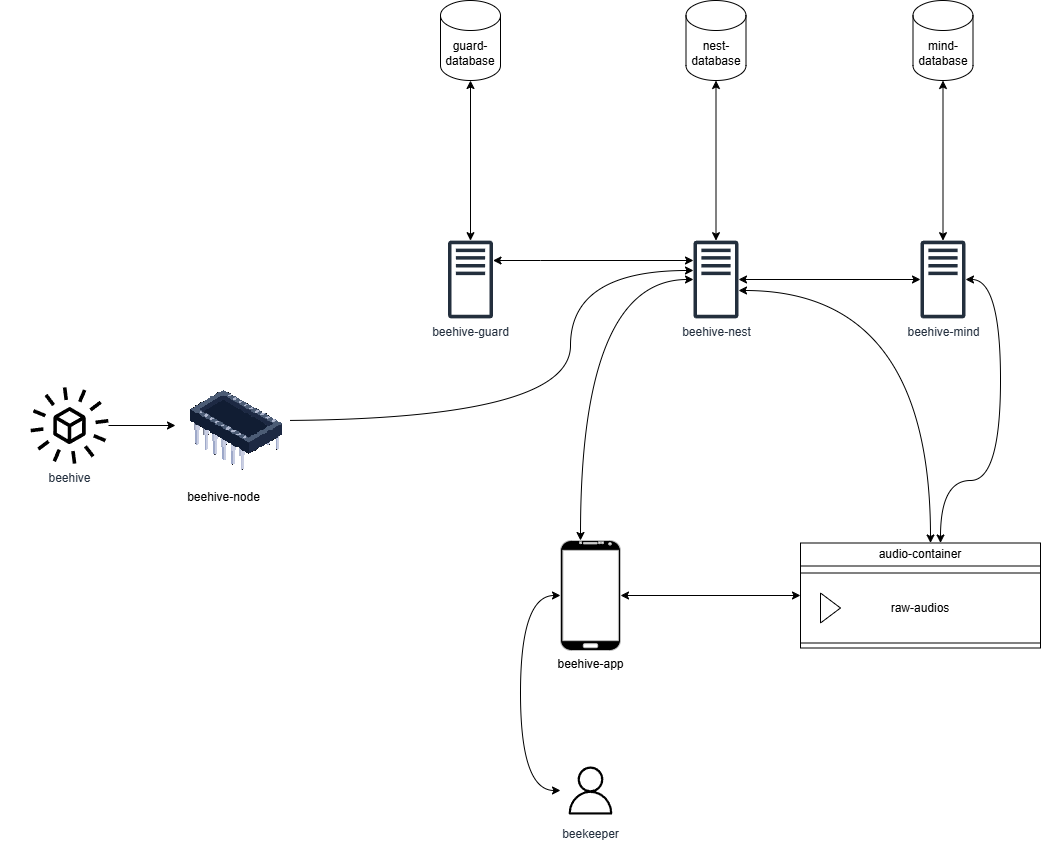
\includegraphics[width=\textwidth]{assets/cap_3/architecture_diagram.png}
    \caption{Arquitectura lógica del sistema propuesto.}
    \label{fig:arquitectura_sistema}
\end{figure}

\begin{table}[H]
    \centering
    \caption{Componentes principales de la arquitectura del sistema}
    \begin{tabular}{@{}lll@{}}
        \toprule
        Componente & Función & Persistencia \\ \midrule
        beehive-node & Captura de datos de sensores & Micro SD \\
        beehive-guard & Autenticación y seguridad & \texttt{PostgreSQL (guard-database)} \\
        beehive-nest & Gestión de metadatos y registros & \texttt{PostgreSQL (nest-database)} \\
        beehive-mind & Análisis de audio con IA & \texttt{PostgreSQL (mind-database)} \\
        audio-container & Almacenamiento de audios crudos &  S3/MinIO (raw-audios) \\
        beehive-app & Interfaz para el apicultor & Local en celular \\ \bottomrule
    \end{tabular}
    \label{tab:componentes_sistema}
\end{table}